\documentclass{article}

\usepackage{geometry}
\usepackage[hidelinks, bookmarks = true]{hyperref}
\usepackage[numbered]{bookmark}
\usepackage{booktabs}
\usepackage{float}
\usepackage{graphicx}
\usepackage{geometry}
\usepackage{titletoc}
\usepackage{indentfirst}
\usepackage{fancyhdr} 
\usepackage{longtable}
\usepackage{supertabular}
\usepackage[normalem]{ulem}
\usepackage{listings}
\usepackage{xcolor}
\usepackage{xurl}
\usepackage{tikz}
\usepackage{lastpage}
\usepackage{amsmath}
\usepackage{amssymb}
\usepackage{mathtools}
\usepackage{caption}
\usepackage{threeparttable}
\usepackage{subcaption}

\geometry{a4paper, left = 1.9cm, right = 1.9cm, top = 2.3cm, bottom = 2.3cm, includehead}
\captionsetup[table]{font={small}}

\pagestyle{fancy}
\fancyhead[R]{\thepage /\pageref{LastPage}}
\fancyhead[L]{GROUP 28}
\fancyfoot{}
\fancyfoot{}
\renewcommand{\headrulewidth}{0pt}
\renewcommand{\footrulewidth}{0pt}
\setlength{\headheight}{14.49998pt}
\addtolength{\topmargin}{-2.49998pt}

\begin{document}
\noindent\rule{\textwidth}{1pt}
\begin{center}
    \LARGE \textbf{Assignment 2: Predict Future Sales}
\end{center}
\noindent\rule{\textwidth}{0.5pt}
\begin{center}
    \textbf{Group 28}\par
    \vspace{0.3cm}
Shuang Fan\phantom{space}Kaiteng Jiang\phantom{space}Shupei Li\\
s3505847\phantom{spacespac}s3479420\phantom{spacespa}s3430863
\end{center}
\textbf{Kaggle team name: AiDM-Group 28}

\section{Algorithms}
This section introduces the best three algorithms we have adopted in the Kaggle competition. Besides, we also explain our evaluation procedure and report the model performance.
\subsection{ARIMA}
The ARIMA model is a traditional statistical method designed for time series data. It combines autoregression and moving average techniques to forecast future trends based on historical observations. Therefore, its input is the previous sales data in this task and doesn't require manually selected features. Compared to sophisticated machine learning models, the ARIMA model is usually more robust and easier to use. We set the ARIMA model as baseline. Since the train set includes nearly two years' daily sales data, we incorporate seasonal terms in ARIMA model. Denoting the time span as $S$, our model can be written in the form of,
\begin{align*}
    ARIMA\left( p, d, q \right) \times\left( P, D, Q \right) S
\end{align*}
where $p$, $d$, $q$ are AR order, difference order, and MA order respectively. And the capital letters correspond to seasonal orders. The target of competition is predicting the monthly sales for each shop-item pair. However, if we create ARIMA models for each shop-item pair, there will be a major difficulty. Although the volume of training data is large, samples amortized for each pair are insufficient to provide enough information about trending to train the ARIMA model. To ensure the validity of ARIMA, we model the monthly sales for each shop and estimate the sales of each item by multiplying the shop sales prediction and the share of the item sales out of total sales. We take shop 2 as an example. Figure \ref{fig:arima-1} is the result of model diagnostics, which supports the model validity. And Figure \ref{fig:arima-2} depicts the original monthly sales data as well as the prediction. According to Figure \ref{fig:arima-2}, the prediction of ARIMA model is reasonable.\par

\begin{figure}[!ht]
    \centering
    \includegraphics[width=10cm]{./figs/arima-1.png}
    \caption{Shop 2: ARIMA Model Diagnostics}
    \label{fig:arima-1}
\end{figure}

\begin{figure}[!ht]
    \centering
    \includegraphics[width=10cm]{./figs/arima-2.png}
    \caption{Shop 2: ARIMA Model Prediction}
    \label{fig:arima-2}
\end{figure}

The standard procedure of creating the ARIMA model is manually setting the parameters related to orders based on model diagnostics. However, it will be laborious if we repeat the parameter selection for all shops. We automate the procedure by using \texttt{auto\_arima} API in pmdarima package. After obtaining shops' monthly sales predictions, we generate the prediction for each shop-item pair with the strategy mentioned before. Items released in November 2015 don't have historical sales data and lead to NaN values. We fill these NaN values with the average value of predictions. RMSE of ARIMA model on test set is 1.18663.

\subsection{Blending Model} \label{method}
Stacking and blending are two commonly used strategies in Kaggle competitions. Model stacking requires cross validation during the training, which may cause information leakage in time series data. Thus, we choose model blending method in our project. Figure \ref{fig:blending} illustrates the model architecture that we design for the dataset.

\begin{figure}[!ht]
    \centering
    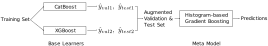
\includegraphics[width=16cm]{./figs/blending.png}
    \caption{Blending: Model Architecture}
    \label{fig:blending}
\end{figure}

Considering the time series nature of the dataset, we select the sales data in October 2015 as validation set and use the data before October 2015 as training set. Firstly, we train two base learners, CatBoost and XGBoost, on training set to obtain predictions on validation set and test set. After that, we regard predictions as new features and merge them into validation set and test set. These augmented data sets are the inputs of the meta model, which is Histogram-based gradient boosting regression tree in our blending model. Specifically, the meta model is fitted on the augmented validation set and output final predictions based on the augmented test set. Table \ref{tab:blending} summarizes the key parameter settings in the blending model. \par

\begin{table}[!ht]
    \centering
    \caption{Blending: Parameter Settings}
    \label{tab:blending}
    \begin{tabular}{lll}
        \toprule
        \textbf{Parameter} & \textbf{Value} & \textbf{Meaning}\\
        \midrule
        early\_stopping\_rounds & 10 & The number of early stopping rounds in CatBoost and XGBoost.\\
        n\_estimators & 5000 & The number of estimators in XGBoost.\\
        max\_depth & 10 & Maximum depth of a tree in XGBoost.\\
        learning\_rate & 0.1 & Learning rate in XGBoost.\\
        subsample & 0.5 & Subsample ratio of the training instances in XGBoost.\\
        \bottomrule
    \end{tabular}
\end{table}

The performance of blending model is better than ARIMA model, whose RMSE on test set is 0.98551.

\subsection{XGBoost}
During the training of blending model, we find that the performance of XGBoost on validation set is better than that of CatBoost. We conjecture using XGBoost alone may produce more accurate predictions. We split the traing data into training set and validation set in the same way as Section \ref{method}. Besides, we use the same parameter settings in Table \ref{tab:blending} for XGBoost. According to results of Kaggle submissions, XGBoost outperforms other two models with 0.93308 RMSE.\par

We perform a feature importance analysis to provide some insights into the effectiveness of XGBoost. F scores of all features can be found in the jupyter notebook. According to the feature importance plot, the median of item's monthly prices and lag values of item's historical sales contribute most to XGBoost's performance.

\subsection{Evaluation Procedure}
RMSE is selected as our metrics, which is consistent with Kaggle. We also clip predictions into the valid range $[0, 20]$. The strategy of generating predictions from the ARIMA model creates a barrier to assess RMSE before submission. As for blending model, we can only infer the model performance from base learners, because the input of the meta model is an augmented version of the validation set. The average of base learners' RMSE is 0.89203. The evaluation of XGBoost model is straightforward, i.e., we can directly calculate RMSE on the validation set. RMSE of XGBoost on validation set is 0.88883. Table \ref{tab:evaluation} summarizes our evaluation results before submission and the real RMSE computed by Kaggle.

\begin{table}[!ht]
    \centering
    \caption{Summary of Evaluation}
    \label{tab:evaluation}
    \begin{tabular}{lll}
        \toprule
        \textbf{Model} & \textbf{Validation RMSE} & \textbf{Test RMSE}\\
        \midrule
        ARIMA & - & 1.18663\\
        Blending Model & 0.89203 & 0.98551\\
        XGBoost & \textbf{0.88883} & \textbf{0.93308}\\
        \bottomrule
    \end{tabular}
\end{table}

\section{Conclusion}
Kaggle competitions with regards to tabular data follow a three-stage workflow: exploratory data analysis, preprocessing and feature engineering, modeling. Exploratory data analysis provides some basic information about data, for example, the existence of missing values or outliers. Plots and descriptive statistics are helpful to avoid disastrous mistakes later in feature engineering and modeling. Preprocessing and feature engineering are higly data-driven. Some information are contained in the text descriptions, e.g. the city appears as the first word in the shop name. Some information are given implicitly and hard to be realized. For instance, the item with zero sales would not be recorded in the training set, which may lead to the bias in model. There are various algorithms for time series data, from the traditional ARIMA to the state-of-the-art XGBoost. The performance of model depends on the quality of features and properties of data. We go through the three-stage process in the project and finally rank in top 35\% on the Kaggle competition.

\end{document}
